

\begin{figure*}[t]
  \centering
  \centering \includegraphics[width=1.0\textwidth]{fig_main.pdf}
  % \fbox{\rule{0pt}{2in} \rule{0.9\linewidth}{0pt}}
   % \includegraphics[width=0.8\linewidth, color=gray]{egfigure.eps}
   \caption{\textbf{Illustrative diagram of the hierarchical block optimization framework.} We first derive a global coarse Gaussian representation using low-resolution data, which is then contracted into a bounded cubic region. Subsequently, the contracted Gaussian primitives are partitioned into blocks, each paired with corresponding data. Leveraging the global coarse Gaussian as initialization, we parallelly refine each block in the original uncontracted space using high-resolution data. During this refinement process, an Importance-Driven Gaussian Pruning strategy is employed to compute the interaction between each Gaussian primitive and training view rays, removing low-contribution primitives to accelerate convergence and reduce redundancy. The optimized blocks are then concatenated to form the final global Gaussian representation, which is validated through novel view synthesis (NVS) and surface reconstruction tasks. }
   \label{fig:main}
\vspace{-0.2cm}
\end{figure*}


\section{Method}
% 写一下各个subsect分别干了啥
Our proposed HRGS efficiently reconstructs high-resolution scenes. 
We first review 3DGS in Section~\ref{3.1}. 
Next, in Section~\ref{3.2}, we present the memory-efficient coarse-to-fine framework, detailing the partitioning of Gaussian primitives and data, along with the proposed Importance-Driven Gaussian Pruning (IDGP) strategy.
%
% Next, in Section~\ref{3.2}, we introduce the memory-efficient coarse-to-fine framework and detail how Gaussian primitives and data are partitioned, {\color{red}as well as the Importance-Driven Gaussian Pruning strategy.}
%
Finally, Section~\ref{3.3} describes the loss function employed in our approach.





\subsection{Preliminary}
\label{3.1}
We begin with a brief overview of 3D Gaussian Splatting (3DGS)~\cite{3dgs}. 
In the 3DGS framework, a scene is represented as a set of discrete 3D Gaussian primitives, denoted by \( G_K = \{ G_k \mid k = 1, \dots, K \} \), where \( K \) is the total number of Gaussians in the scene. 
Each Gaussian \( G_k \) is defined by a set of learnable parameters, including its 3D position \( \mathbf{p}_k \in \mathbb{R}^{3 \times 1} \), opacity \( \sigma_k \in [0, 1] \), and geometric properties, which typically consist of scaling and rotation parameters that define the Gaussian covariance matrix \( \Sigma_k \in \mathbb{R}^{3 \times 3} \). %i.e. \( \Sigma_k = \mathbf{R}_k \mathbf{S}_k \mathbf{S}_k^\top \mathbf{R}_k^\top \). 
Furthermore, spherical harmonic (SH) features \( f_k \in \mathbb{R}^{3 \times 16} \) are used to encode view-dependent color information \( c_k \in \mathbb{R}^{3 \times 1} \), allowing for a realistic depiction of color variations as a function of the viewing angle.

For rendering purposes, the combined color and opacity contributions from multiple Gaussians at a given pixel are weighted according to their respective opacities. The color blending for overlapping Gaussians is computed as follows:
\begin{equation}
\hat{C} = \sum_{k \in M} c_k \alpha_k \prod_{j=1}^{k-1} \left( 1 - \alpha_j \right),
\label{eq1}
\end{equation}
where \( c_k \) and \( \alpha_k = \sigma_kG_k \) denote the color and density of the \( k \)-th Gaussian primitive, respectively.

% \begin{figure*}[htp]
%   \centering
%   \centering \includegraphics[width=1.0\textwidth]{fig_main.png}
%   % \fbox{\rule{0pt}{2in} \rule{0.9\linewidth}{0pt}}
%    % \includegraphics[width=0.8\linewidth, color=gray]{egfigure.eps}
%    \caption{\textbf{Illustrative diagram of the hierarchical block optimization framework.} We first derive a global coarse Gaussian representation using low-resolution data, which is then contracted into a bounded cubic region. Subsequently, the contracted Gaussian primitives are partitioned into blocks, each paired with corresponding data. Leveraging the global coarse Gaussian as initialization, we parallelly refine each block in the original uncontracted space using high-resolution data. During this refinement process, an Importance-Driven Gaussian Pruning strategy is employed to compute the interaction between each Gaussian primitive and training view rays, removing low-contribution primitives to accelerate convergence and reduce redundancy. The optimized blocks are then concatenated to form the final global Gaussian representation, which is validated through novel view synthesis (NVS) and surface reconstruction tasks. }
%    \label{fig:main}
% \vspace{-0.2cm}
% \end{figure*}

\subsection{Hierarchical Block Optimization Framework}  
\label{3.2}

Traditional 3D Gaussian methods~\cite{3dgs,vcR} rely on global iterative optimization for scene reconstruction but struggle with memory inefficiency in high-resolution settings, such as the Mip-NeRF 360~\cite{mip} dataset. To address this, we propose a hierarchical optimization framework that balances coarse global representation and fine-grained local refinement, as shown in Fig~\ref{fig:main}. We first construct a low-resolution global Gaussian prior, guiding block-wise high-resolution optimization to enhance geometric detail while maintaining memory efficiency. This approach enables precise reconstruction under constrained memory conditions. The following subsections detail the coarse global Gaussian generation, Gaussian and data partitioning strategies, as well as refinement and post-processing procedures.

\noindent\textbf{Coarse Global Gaussian Representation.}
This stage establishes the foundation for subsequent Gaussian and data partitioning. Initially, we train the COLMAP~\cite{schoenberger2016mvs,schoenberger2016sfm} points using all observations at a low resolution for 30,000 iterations, generating a coarse representation of the global geometric structure. The resulting Gaussian primitives are represented as \( G_K = \{ G_k \mid k = 1, \ldots, K \} \), where \( K \) denotes the total number of Gaussians. In the following block-wise high-resolution refinement, this robust global geometric prior ensures that Gaussians are positioned accurately, thereby preventing drift and eliminating inter-block discontinuities, minimizing significant fusion artifacts.

\noindent\textbf{Primitives and Data Division.}
Directly applying uniform grid division in the original 3D space may lead to uneven Gaussian distribution in local regions (e.g. many nearly empty grid cells alongside overly dense ones). 
% \textcolor{red}{
% To avoid this imbalance, the coarse global Gaussian prior is first contracted to a bounded cubic region.
% For contraction, we define a internal region in the central one-third of the space with the minimum and maximum positions of its corners $\mathbf{p}_{\text{min}}$ and $\mathbf{p}_{\text{max}}$.
% The remainder of the space is then designated as the external region.
% To mitigate this imbalance, we first define a bounded cubic region and contract all Gaussians toward it.
% Within this cubic region, central one-third of the space bounded by minimum and maximum positions of its corners $\mathbf{p}_{\text{min}}$ and $\mathbf{p}_{\text{max}}$, is designated as the internal region, while the remainder is classified as the external region.
%The remainder of the space is then designated as the external region.
To address this imbalance, we define a bounded cubic region and contract all Gaussians within it. Within this region, the central one-third of the space is designated as the internal region, while the surrounding area is classified as the external region. The internal region is bounded by the minimum and maximum corner positions, $\mathbf{p}_{\text{min}}$ and $\mathbf{p}_{\text{max}}$, which define the limits of the central one-third of the entire region.
% }
To standardize the representation of global Gaussians, we introduce a normalization step:
\(
\hat{\mathbf{p}}_k =  2\left( {\mathbf{p}_k - \mathbf{p}_{\text{min}}}\right)/\left({\mathbf{p}_{\text{max}} - \mathbf{p}_{\text{min}}} \right)-1.
\)
As a result, the coordinates of Gaussians located in the internal region are constrained within the range $[-1, 1]$. 
To achieve more effective contraction of the global Gaussians, we apply a linear mapping for the Gaussians in the internal region, while a nonlinear mapping is employed for the external region (as shown in Fig.~\ref{fig:main}). The final contraction step is performed using the function described in \cite{scanerf}:
\small{
    \begin{equation}
        % \small
        \text{contract} (\hat{\mathbf{p}}_k) =
        \begin{cases}
        \hat{\mathbf{p}}_k, & \text{if } \|\hat{\mathbf{p}}_k\|_\infty \leq 1, \\
        \left( 2 - \frac{1}{\|\hat{\mathbf{p}}_k\|_\infty} \right) \frac{\hat{\mathbf{p}}_k}{\|\hat{\mathbf{p}}_k\|_\infty}, & \text{if } \|\hat{\mathbf{p}}_k\|_\infty > 1.
        \end{cases}
        \label{12}
    \end{equation}
}
The contracted space is then uniformly partitioned into $n$ blocks (the specific number of blocks used will be discussed further in Sec.~\ref{experiments}.), resulting in a more balanced Gaussian partitioning.
After partitioning the Gaussians, our objective is to ensure that each block is sufficiently trained. In other words, the training data assigned to each block should be highly relevant to the region it represents, focusing on refining the details within the block. To achieve this, we select observations and retain only those that contribute significantly to the visible content of the corresponding block in the rendering results. Since SSIM loss effectively captures structural differences and is somewhat robust to brightness variations~\cite{mss}, we use it as the foundation for our data partition strategy. Specifically, for the $j$-th block, the global Gaussians contained within it are represented as:
\(
G_{Kj} = \{ G_k \mid b_{j, \text{min}} \leq \text{contract}(\hat{\mathbf{p}}_k) < b_{j, \text{max}}, k = 1, \dots, K_j \},
\)
where $b_{j, \text{min}}$ and $b_{j, \text{max}}$ define the spatial bounds of the $j$-th block, and $K_j$ is the number of Gaussians contained within the block. 
%Whether the $i$-th pose $\tau_i$ is assigned to the $j$-th block is determined by the following condition:
The set of observations assigned to the \(j\)-th block is defined by the following formula:
\small{
\begin{equation}
\begin{aligned}
    \mathbf{P}^1_j = \text{Mask}\left(\mathcal{L}_{\text{SSIM}} \left( I_{G_K} (\boldsymbol{\tau}), I_{G_K \setminus G_{Kj}} (\boldsymbol{\tau}) \right ) > \epsilon \right )
    \odot \boldsymbol{\tau},
\end{aligned}
\label{13}
\end{equation}
}
where \( \text{Mask}(\cdot) \) generates an element-wise binary mask. Each element of the mask is set to 1 if it satisfies the condition inside the mask (i.e. the SSIM loss exceeds a threshold \( \epsilon \)), and 0 otherwise.
The term \( G_K \setminus G_{Kj} \) denotes the portion of the global set \( G_K \) excluding the block \( G_{Kj} \). \( \boldsymbol{\tau} \) is a matrix containing all camera poses, with each column \( \tau_i \) representing the \( i \)-th camera pose.
\( \odot \) is element-wise product operation.
And the resulting set \( \mathbf{P}^1_j \) represents the camera poses assigned to the \( j \)-th block. 
%Where $G_K \setminus G_{Kj}$ denotes the portion of $G_K$ that does not include $G_{Kj}$. The $i$-th pose $\tau_i$ is assigned to the $j$-th block only when the SSIM loss $L_{\text{SSIM}}$ exceeds a threshold $\epsilon$. 



However, this strategy does not account for the projection of the considered block, which may lead to artifacts at the edges of the block. To address this issue, we further include poses that fall within the boundaries of the considered block:
\begin{equation}
    \mathbf{P}^2_j = \text{Mask}\left(b_{j, \text{min}} \leq \text{contract} (\hat{\mathbf{p}}_{\tau_i}) < b_{j, \text{max}} \right) \odot \boldsymbol{\tau}.
\label{14}
\end{equation}
where $\hat{\mathbf{p}}_{\tau_i}$ is the position under the world coordinate of pose $i$. The final assignment is:
% \begin{equation}
%     B_2 (\tau_i, G_{Kj}) =
%     \begin{cases}
%     1, & b_{j, \text{min}} \leq \text{contract} (\hat{\mathbf{p}}_{\tau_i}) < b_{j, \text{max}}, \\
%     0, & \text{otherwise}.
%     \end{cases}
% \label{14}
% \end{equation}

% \begin{equation}
%     \mathbf{P}^2_j = \text{Mask}\left(b_{j, \text{min}} \leq \text{contract} (\hat{\mathbf{p}}_{\tau_i}) < b_{j, \text{max}} \right) \odot \boldsymbol{\tau}.
% \label{14}
% \end{equation}
% where $\hat{\mathbf{p}}_{\tau_i}$ is the position under the world coordinate of pose $i$. The final assignment is:
% \begin{equation}
%     \mathbf{P}_j(\boldsymbol{\tau}, G_{Kj}) = \mathrm{Merge}\bigl(\mathbf{P}^1_j, \mathbf{P}^2_j\bigr),
% \end{equation}
% where $\mathrm{Merge}$ denotes the concatenate operator that removes any duplicate elements, ensuring only one copy of each element is retained.

% \begin{figure*}[h]
%   \centering
%   \centering 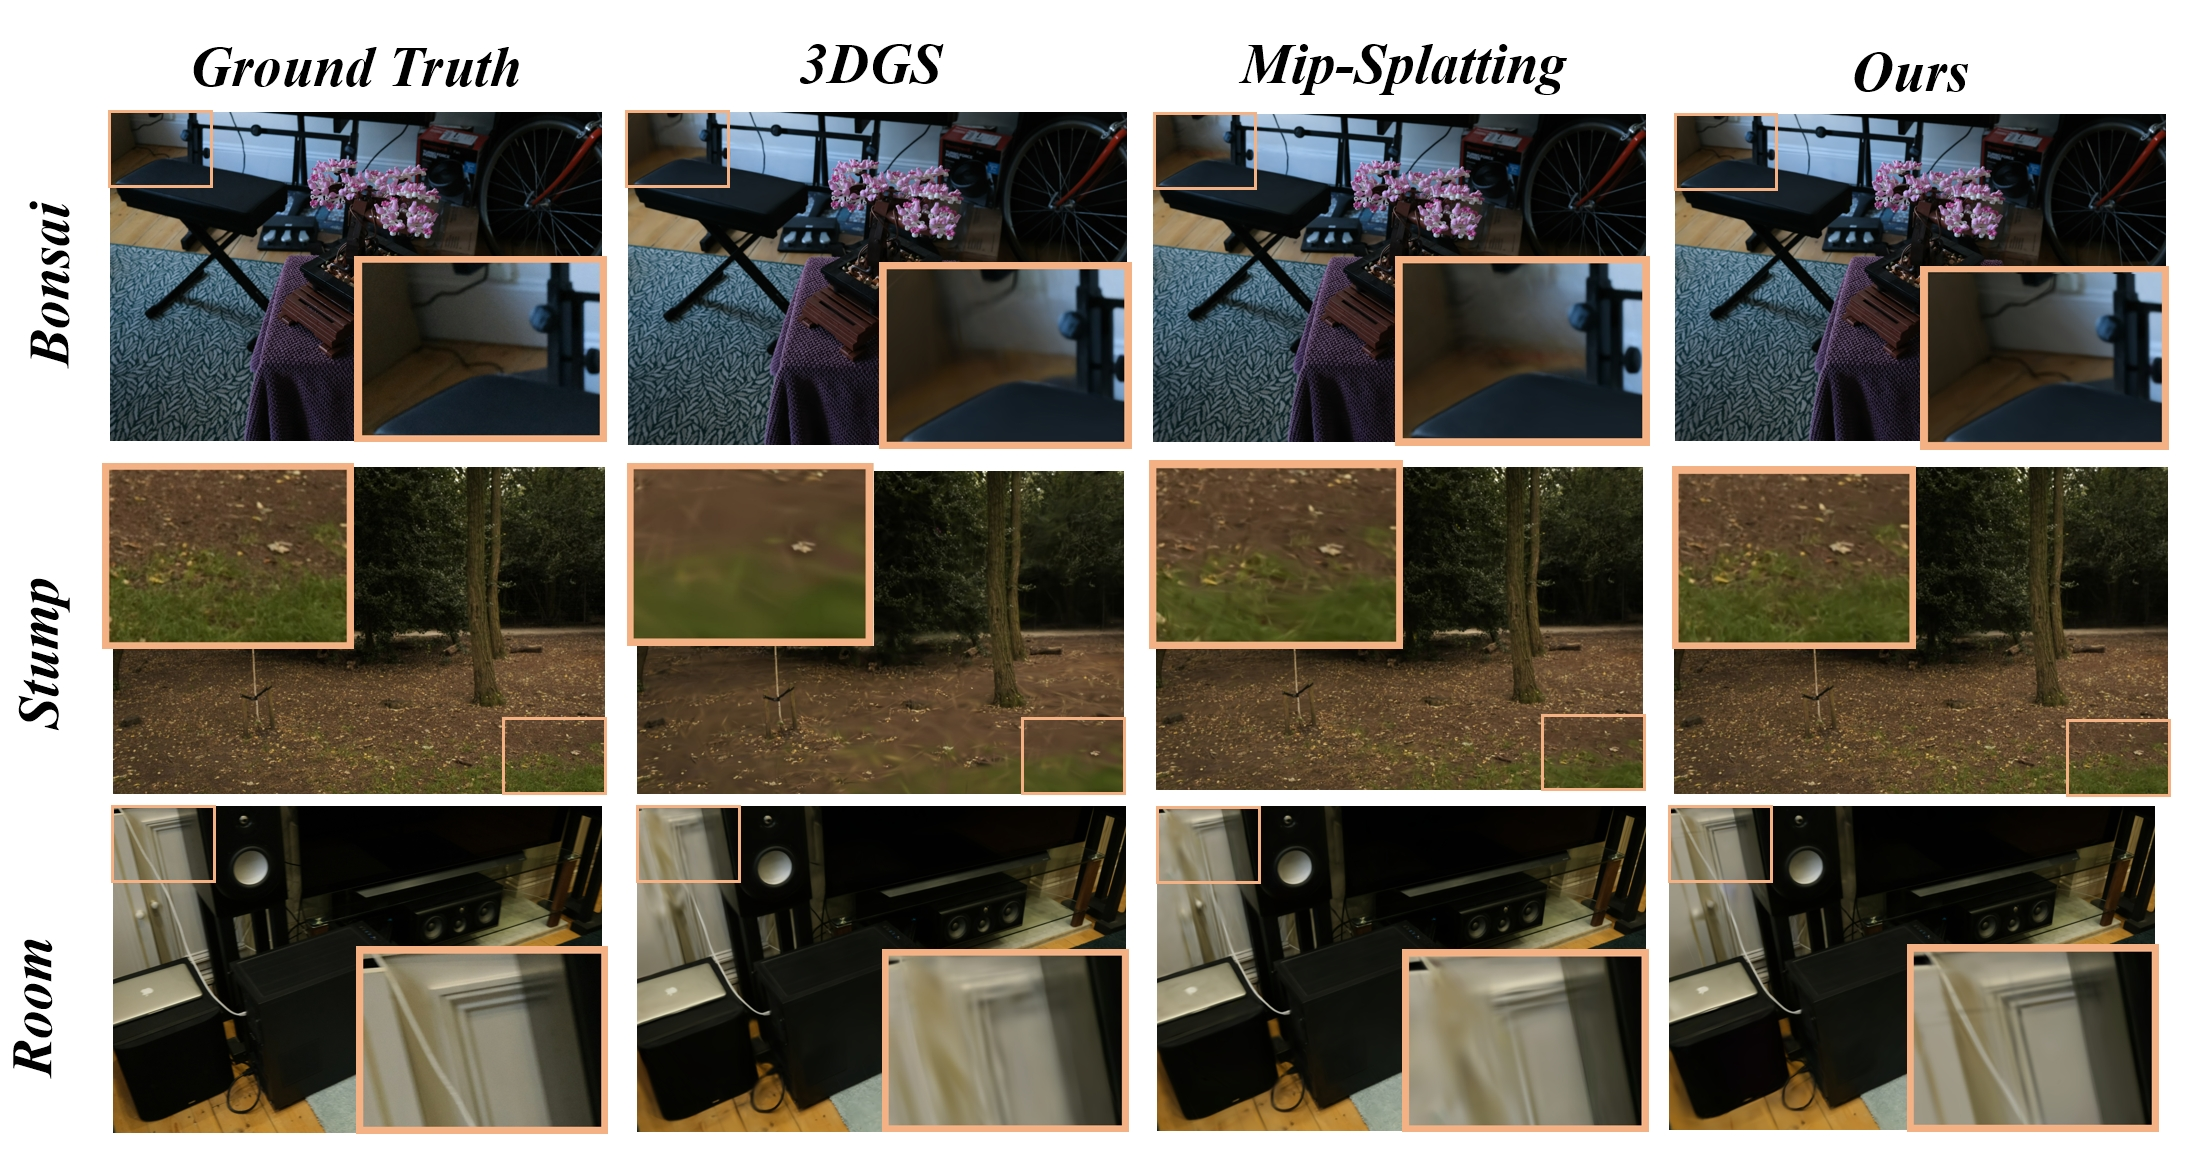
\includegraphics[width=1.0\textwidth]{fig3.png}
%   % \fbox{\rule{0pt}{2in} \rule{0.9\linewidth}{0pt}}
%    % \includegraphics[width=0.8\linewidth, color=gray]{egfigure.eps}
%   \caption{%
%     \textbf{\textcolor{red}{Qualitative Comparison on the Mip-NeRF 360 Dataset. }}%
% Three representative scenes demonstrate that our method more faithfully preserves fine-scale structures and achieves superior visual fidelity compared to 3DGS and Mip-Splatting.
%   }
%    \label{fig:4}
% \end{figure*}
\begin{equation}
    \mathbf{P}_j(\boldsymbol{\tau}, G_{Kj}) = \mathrm{Merge}\bigl(\mathbf{P}^1_j, \mathbf{P}^2_j\bigr),
\end{equation}
where $\mathrm{Merge}$ denotes the concatenate operator that removes any duplicate elements, ensuring only one copy of each element is retained.


To prevent overfitting, we employ a binary search method~\cite{binary} to incrementally expand $b_{j, \text{min}}$ and $b_{j, \text{max}}$ until $K_j$ exceeds a predefined threshold. 
Notably, this procedure is applied exclusively during the data partitioning phase for each block.


\noindent\textbf{Importance-Driven Gaussian Pruning (IDGP).}
After the Gaussian primitives and data division, we proceed to train each block in parallel in the original uncontracted space. Specifically, we first initialize each block using the coarse global Gaussian prior, and then fine‐tune each block using high‐resolution data as detailed in Sec.~\ref{3.3}. During block‐level optimization, we further accelerate convergence and reduce redundancy by applying a lightweight importance scoring and pruning strategy. Let $\mathcal{R}_b$ denote the set of all rays cast from the training views assigned to block $b$. For each Gaussian primitive $p_i$ in block $b$, we only consider its interactions with $\mathcal{R}_b$ and define the weighted hit count as
\small{
\begin{equation}
H_i \;=\;\sum_{r\in\mathcal{R}_b}\mathbf{1}(p_i \cap r)\,T_{i,r},
% \end{equation}
% \begin{equation}
\text{where } T_{i,r} =\prod_{\substack{p_k \cap r\\\mathrm{depth}(p_k)<\mathrm{depth}(p_i)}}\bigl(1 - \alpha_k\bigr).
\end{equation}
}
Here, $\mathbf{1}(p_i \cap r)=1$ if and only if ray $r$ intersects $p_i$, and $T_{i,r}$ accumulates the transmission up to $p_i$ by all closer primitives $p_k$. We then compute the raw volume of $p_i$ as
\small{
$
v_i \;=\;\prod_{d=1}^3 s_{i,d},
$}
where each \(s_{i,d}\) is the scale factor of $p_i$ along the $d$-th spatial axis, and apply logarithmic compression
$
\widetilde{v}_i \;=\;\ln\bigl(1 + v_i\bigr).
$
Finally, we assign each primitive an importance score with its opacity $\alpha_i$:
$
S_i \;=\;\alpha_i\;\widetilde{v}_i\;H_i.
$
After evaluating $\{S_i\}$ for all primitives in the block, we sort them in descending order and remove the lowest 20\%. The remaining Gaussians, now both globally informed by the coarse prior and locally pruned of low‐impact points, continue through block‐level fine‐tuning. Finally, we select the fine‐tuned Gaussians within each block and, guided by the global geometric prior, concatenate the blocks to obtain the fine‐tuned global Gaussian. Through this process, the previously coarse global Gaussians are significantly enhanced in areas where they lacked detail.








\subsection{Loss Function}  
\label{3.3}
To optimize both the coarse and refined stages,the loss functions are defined as follows. First, we use the RGB loss $\mathcal{L}_{RGB}$ from 3DGS for the novel view synthesis task. To reconstruct scene surfaces, we enforce normal priors $\mathbf{N}$ predicted by a pretrained monocular deep neural network~\cite{BaeD24} to supervise the rendered normal map $\hat{\mathbf{N}}$ using $\mathbf{L1}$ and cosine losses:

\begin{equation}
    \mathcal{L}_n = \| \hat{\mathbf{N}} - \mathbf{N} \|_1 + (1 - \hat{\mathbf{N}} \cdot \mathbf{N}).
\label{eq2}
\end{equation}







Additionally, to effectively update Gaussian positions, we utilize the predicted normal $\mathbf{N}$ from the pretrained model to supervise the D-Normal $\overline{\mathbf{N}}_d$. The D-Normal is derived from the rendered depth by computing the cross-product of horizontal and vertical finite differences from neighboring points:

\begin{equation}
\overline{\mathbf{N}}_d = \frac{\nabla_v \mathbf{d} \times \nabla_h \mathbf{d}}{\left|\nabla_v \mathbf{d} \times \nabla_h \mathbf{d}\right|},
\label{eq5}
\end{equation}
where $\mathbf{d}$ represents the 3D coordinates of a pixel obtained via back-projection from the depth map. We then apply the D-Normal regularization from ~\cite{vcR}:

\begin{equation}
    \mathcal{L}_{dn} = w \cdot \left(\| \bar{\mathbf{N}}_d - \mathbf{N} \|_1 + (1 - \bar{\mathbf{N}}_d \cdot \mathbf{N})\right),
\label{eq8}
\end{equation}
where $w$ is a confidence term. The overall loss function integrates these components:

\begin{equation}
    \mathcal{L}_{total} = \mathcal{L}_{RGB} + \lambda_1 \mathcal{L}_s + \lambda_2 \mathcal{L}_n + \lambda_3 \mathcal{L}_{dn},
\label{eq9}
\end{equation}
where $\lambda_1$, $\lambda_2$, and $\lambda_3$ balance the individual terms. The term $\mathcal{L}_s$ is introduced to simplify depth computation, as described in~\cite{vcR}.





\begin{figure*}[t]
  \centering
  \centering 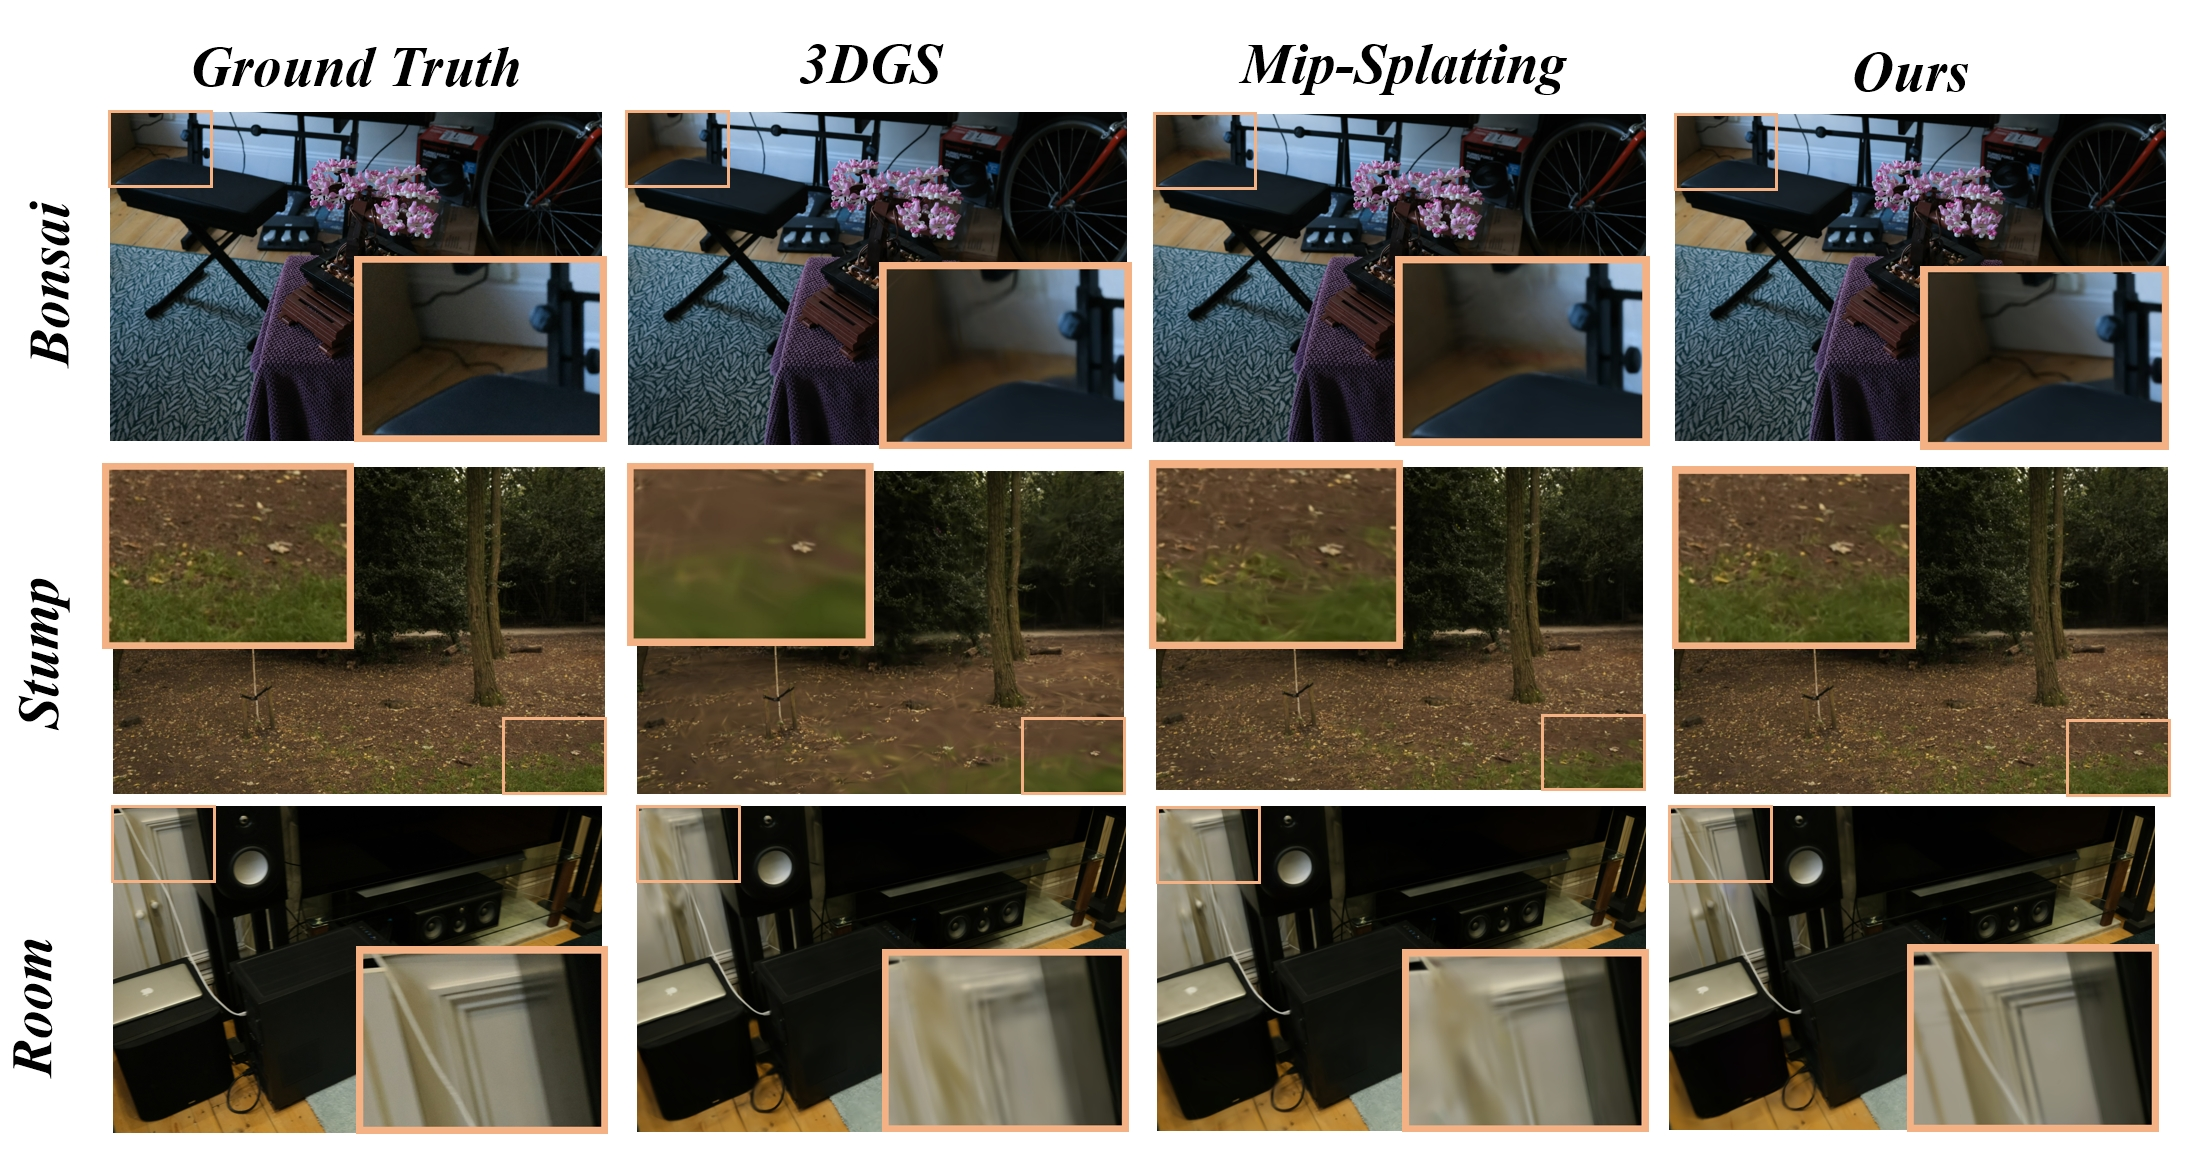
\includegraphics[width=1.0\textwidth]{fig3.pdf}
  % \fbox{\rule{0pt}{2in} \rule{0.9\linewidth}{0pt}}
   % \includegraphics[width=0.8\linewidth, color=gray]{egfigure.eps}
  \caption{%
    \textbf{Qualitative Comparison on the Mip-NeRF 360 Dataset. }%
Three representative scenes demonstrate that our method more faithfully preserves fine-scale structures and achieves superior visual fidelity compared to 3DGS and Mip-Splatting.
  }
   \label{fig:4}
   % \vspace{-0.2cm}
\end{figure*}